\documentclass[../CHEFCookingHelper.tex]{subfiles}

\begin{document}

% Flush bottom doesn't work well with just floats
\raggedbottom

\begin{table}[h!]
    \centering
    \begin{tabular}{cc}\toprule
        \multicolumn{2}{c}{KV6003: Individual Computing Project Student eLogbook} \\\midrule
        Student name and ID & Kieran Knowles w20013000 \\
        Academic year & 2023--2024 \\
        Programme: & Pure Computer Science \\
        Project title & \chef{} \\
        Supervisor & Nick Dalton \\
        Supervisor email and room number & \makecell[c]{
            CIS 304 \\
            \href{mailto:nick.dalton@northumbria.ac.uk}{nick.dalton@northumbria.ac.uk}
        } \\
        Second marker & Marta Cecchinato \\
        Second marker email and room number & \makecell[c]{
            CIS 307 \\
            \href{mailto:marta.cecchinato@northumbria.ac.uk}{marta.cecchinato@northumbria.ac.uk}
        } \\\bottomrule
    \end{tabular}
\end{table}

\textbf{\underline{PROJECT E LOGBOOK INSTRUCTIONS}}

This eLogbook can be used to record the progress of work on the project. It covers all the stages of the
work, and it is strongly recommended that it be \ul{completed in full by the student.}

\textit{
    Note: if this eLogbook is not used by the student, \ul{a suitable alternative should be adopted in agreement with
    the Project Supervisor;} the alternative should be accessible by the project tutor if the need arises and able
    to be included as electronic appendices in the final dissertation submission (e.g., consider how the alternative
    can be exported).
}

This eLogbook or other form of project log should be submitted upon completion of the project.
You should also use excerpts from it to evidence claims made in the evaluation section of your report.

\textbf{BEFORE EACH MEETING}

Before each meeting, \textbf{\ul{YOU} must complete the following sections of the relevant weekly log form
(\colorbox{\logbookshadecolour}{shaded in orange}) and \ul{SHARE} the revised complete eLogbook with your Supervisor
(e.g., via email, shared file space):}

\begin{itemize}
    \item Date and time of the meeting;
    \item Brief description of work done since the last meeting;
    \item Number of hours spent on the project since the last meeting;
    \item Questions/items to discuss at the meeting (agenda).
\end{itemize}

\textbf{AFTER EACH MEETING}

\textbf{By the end of the meeting, YOU and your SUPERVISOR must complete the other parts of the form for the week
(not shaded).} After the remaining sections are completed during the meeting, the revised eLogbook should be once
again saved and shared (i.e., via email or shared file space).

If, for any reason, you have more than one meeting in a week or hold a meeting outside of teaching weeks,
simply copy and paste a blank table to create a new entry, taking care to place it in chronological order and
change the heading to something meaningful. For example, if you have two meetings in one week you could use
Week 3a and Week 3b or Week 3.1 and Week 3.2 to indicate the occurrences; alternatively, if you meet outside
allocated teaching weeks for any reason, you could add the meeting date to the heading.

It is recommended that you use the \enquote*{Navigation Pane} in Word to provide easy and quick access to each respective
log form and/or other component.  On the top menu, simply select \enquote*{View} and tick the \enquote*{Navigation Pane} box, which
is located in the \enquote*{Show} section towards the left-hand side.

Note that the time spent column is very approximate.

\logbookentry
{Semester 1 Week 5a}
{Thursday 2nd November 16:00--17:00}
{Begin working on the TOR and ethics approval and start the competitor analysis in the main report}
{N/A}
{What needs to be said in the Data Collection and Data Management sections of the ethics approval? Can I use customer reviews as a data source?}
{Finalize the TOR and ethics approval.}
{TOR and ethics approval}
{Friday 3rd November 11:05--11:35}
{Yes}

\logbookentry
{Semester 1 Week 5b}
{Friday 4th November 11:05--11:35}
{Finalize the ethics approval and complete most of the terms of reference.}
{2 hours.}
{Review the TOR and submit it for review. Clarify which referencing style to use. Begin work on implementing the project.}
{Finish and submit the terms of reference. Add machine learning to group similar recipes and suggest them.}
{The TOR needs to do something different to existing products such as incorporating machine learning.}
{Thursday 9th November 16:00--17:00}
{Yes}

\logbookentry{Semester 1 Week 6}
{Thursday 9th November 16:00--17:00}
{Start implementing the app by getting data imported.}
{5 hours}
{N/A}
{Complete data import and make a start on tracking ingredients.}
{App backend.}
{Thursday 16th November 16:00--17:00}
{Yes}

\logbookentry{Semester 1 Week 7}
{Thursday 16th November 16:00--17:00}
{Get the data import to a state I'm happy with.}
{15 hours.}
{N/A}
{Get ingredient tracking and recipe suggestions implemented.}
{Data import component of the app.}
{Thursday 30th November 16:00--17:00}
{Yes}

\logbookentry{Semester 1 Week 9}
{Thursday 30th November 16:00--17:00}
{Implement basic recipe suggestion}
{10 hours.}
{How should sources for programming be cited?}
{Design and make a start on implementing the front end. Look into unit testing and machine learning for recipe suggestions using a single-layer perceptron model.}
{N/A}
{Thursday 7th December}
{Yes}

\logbookentry
{Semester 1 Week 10}
{Thursday 7th December 16:00--17:00}
{Start implementing the front end. The user can view their ingredients, add ingredients manually, and view available recipes.}
{20 hours.}
{Can copilot be used for generating code?}
{Continue working on the app. Look further into unit testing.}
{Frontend app. Copilot can be used for the code.}
{Thursday 14th December}
{Yes}

\logbookentry
{Semester 1 Week 11}
{Thursday 14th December 16:00--17:00}
{Show the ingredients required for a recipe. Allow filtering to allow one or more missing ingredients. Check ingredient amounts.}
{10 hours.}
{N/A}
{Run machine learning in Node rather than Python.}
{Backend.}
{Thursday 21st December}
{Yes}

\logbookentry
{Semester 1 Week 12}
{Thursday 21st December 16:00--17:00}
{Implement machine learning into the app to find similar recipes. Start documenting ML implementation.}
{15 hours.}
{N/A}
{Complete the app and start testing.}
{App}
{Thursday 1st February 16:00--17:00}
{Yes}

\logbookentry
{Semester 2 Week 1}
{Thursday 1st February 16:00--17:00}
{Finish the app to a state I'm happy with.}
{100 hours.}
{N/A}
{Start work on the report. Start with what is easiest to write and aim for 1000 words
per week. The testing part is how the project is evaluated, in my case, how effective
it appears to be, and the effectiveness of the unit tests.}
{App}
{Thursday 8th February 16:00-17:00}
{Yes}

\logbookentry
{Semester 2 Week 2}
{Thursday 8th February 16:00-17:00}
{Work on the practical work section of the report. Done about 750 words.}
{5 hours.}
{N/A}
{Look into data that can be obtained from the app. How effective is the
comparison of similar recipes? Are nonsensical recipes suggested alongside
correct data?}
{Report, backend of app.}
{Thursday 15th February 16:00-17:00}
{Yes}

\logbookentry
{Semester 2 Week 3}
{Thursday 15th February 16:00-17:00}
{Work on results section of the report and add more test cases. Done about 500 words and at 2800.}
{5 hours.}
{N/A}
{Test that embeddings return higher similarities for more similar recipes.
Look into using Hemmingway to check readability.}
{Report}
{Thursday 22nd February 16:00-17:00}
{Yes}

\logbookentry
{Semester 2 Week 4}
{Thursday 22nd February 16:00-17:00}
{Add some test cases and do a small amount of report work, primarily on the results
section. Done 300 words, now at 3100.}
{8 hours.}
{N/A}
{Continue working on report. Focus on analysing data and on things that will add to the thesis.}
{Report}
{Thursday 29th February 16:00-17:00}
{Yes}

Overall report structure should be:
\begin{itemize}
    \item Abstract
    \item Introduction
    \item Research and planning
    \item Literature Review
    \item Methodology
    \item Design
    \item Evaluation
    \item Findings
    \item Product
    \item Project Process
    \item Conclusion
\end{itemize}

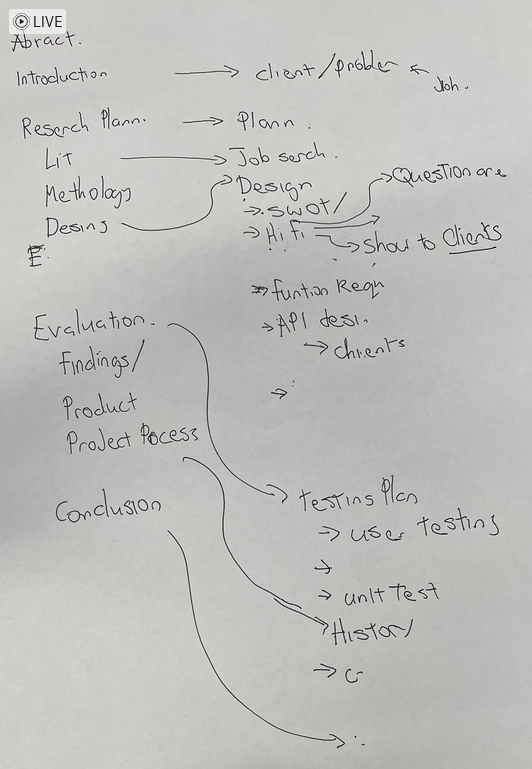
\includegraphics[angle=90,width=\textwidth]{appendicies/report_structure.png}

\logbookentry
{Semester 2 Week 5}
{Thursday 29th February 16:00-17:00}
{Finish writing up about unit testing, make a start on the literature review.
Done 450 words, now at 3550.}
{6 hours.}
{TODO: Questions/items to discuss at the meeting}
{Continue work on literature review. Focus more on AI recipe suggestion rather than
food waste.}
{Literature Review}
{Thursday 7th March 16:00-17:00}
{Yes}

\logbookentry
{Semester 2 Week 6}
{Thursday 7th March 16:00-17:00}
{Done tiny bit of literature review on the use of AI in recipe suggestions (not the most relevant to this project)
Done 100 words, now at 3650}
{2 hours.}
{}
{}
{}
{Thursday 14th March 16:00-17:00}
{Yes}

\logbookentry
{Semester 2 Week 7}
{Thursday 14th March 16:00-17:00}
{Tiny bet of work on literature review. Done 250 words, now at 3900.}
{2 hours.}
{N/A}
{Explain why not trying it on people. Do this in methodology and discuss how I'm more interested in the results than what people are saying about it. This is a
more algorithmic thesis. Write in the style of prior papers.}
{Still on track for the deadline (aiming for 8000 words total). The literature review is the slowest part to work on.}
{Thursday 21st Match 16:00-17:00}
{Yes}

\logbookentry
{Semester 2 Week 8}
{Thursday 21st March 16:00-17:00}
{Very little work done as I have been focusing on the team project. Done 200 words, now at 4100.}
{4 hours.}
{N/A}
{Continue work on report. Consider changing marking scheme to focus primarily on code.}
{Report}
{After Easter}
{Yes}

\logbookentry
{Semester 2 Week 9 (After Easter)}
{Thursday 18th April 16:00-17:00}
{Work on practical work sections of the report. Done 500 words, now at 4600.}
{15 hours.}
{What should I focus on?}
{Continue work on the report.}
{Report}
{Thursday 25th April 16:00-17:00}
{Yes}

\logbookentry
{Semester 2 Week 10}
{Thursday 25th April 16:00-17:00}
{Work on the practical work section of the report, mainly implementation and testing.
Done 1100 words, now at 5700.}
{8 hours.}
{How do I go about changing the marking scheme? What should I change it to?
Should use case diagrams be in the main report or the appendix?}
{Keep use case diagrams in the appendix. Send current draft for review, focusing on
the literature review and how recipe similarity has been evaluated before.}
{Report}
{Thursday 2nd May 16:00-17:00}
{Yes}

\logbookentry
{Semester 2 Week 11}
{Thursday 2nd May 16:00-17:00}
{Restructure report following feedback. Done 550 words, now at 6250.}
{5 hours.}
{None}
{Get things done ready for the deadline. Can get some last-minute feedback if needed.}
{Report}
{N/A - this was the last meeting.}
{Yes, but cut short.}

\end{document}
